\documentclass[11pt]{article}
\usepackage[margin=1in]{geometry}
\usepackage{amsmath,amssymb}
\usepackage{graphicx}
\usepackage{url}
\usepackage{booktabs}
\usepackage{array}
\usepackage{caption}
\usepackage{float}
\usepackage[T1]{fontenc}
\usepackage{lmodern}
\captionsetup{font=small,labelfont=bf}
\setlength{\parskip}{2pt}
\newcommand{\betai}{\hat{\beta}_{i}}
\usepackage{listings}
\usepackage{xcolor}
\definecolor{codebg}{rgb}{0.975,0.975,0.975}
\definecolor{codekw}{rgb}{0.10,0.25,0.55}
\definecolor{codecm}{rgb}{0.20,0.45,0.35}
\definecolor{codestr}{rgb}{0.45,0.30,0.10}
\lstdefinestyle{py}{
  language=Python,
  basicstyle=\ttfamily\footnotesize\linespread{1.0}\selectfont,
  keywordstyle=\color{codekw}\bfseries,
  commentstyle=\color{codecm}\itshape,
  stringstyle=\color{codestr},
  numberstyle=\tiny\color{gray},
  numbers=left, numbersep=6pt, stepnumber=1,
  breaklines=true, breakatwhitespace=false,
  showstringspaces=false, tabsize=4,
  frame=single, rulecolor=\color{gray!50},
  framexleftmargin=12pt, framextopmargin=4pt, framexbottommargin=4pt,
  backgroundcolor=\color{codebg},
  aboveskip=8pt, belowskip=14pt,
  upquote=true, columns=fullflexible, keepspaces=true
}
\lstset{style=py}
\begin{document}

\begin{center}
{\LARGE\bfseries Bank Interest-Rate Sensitivity\\[4pt]
\large Reproducible Empirical Analysis of U.S. Commercial Banks, 1984--2017}\\[10pt]
Cunhan Guo
\end{center}

\noindent\textbf{Reproducibility.} The scripts in \texttt{code/} read the four
raw files under \texttt{data/} and write processed data, tables, and figures
under \texttt{data\_processed/} and \texttt{output/}. Run scripts 01 through
06 in order from the project root. The bank-quarter panel spans
1984Q1--2017Q4.

\section{Data Audit and Descriptive Evidence}

\subsection{Data and data-preparation choices}
Four files are provided. \path{callreports_1984_2017.dta} holds
1,114,194 bank-quarter rows for 17,804 distinct commercial-bank identifiers,
calendar quarter, quarterly average assets, total interest income, total
interest expense, and net income. After excluding rows with missing flows or
non-positive assets, 17,743 banks remain with at least one usable quarter;
61 raw identifiers have no usable observations. \texttt{FedFunds.csv} is the monthly
effective federal funds rate; I take the last month of each quarter as
$f_t$. \path{Bank_and_CRSP_Linking_Table.csv} and
\path{CRSP_Monthly_Stock_File.csv} are used in Section~\ref{sec:stocks}.

The three income/expense/net-income items are year-to-date (YTD) cumulative
flows, not single-quarter flows. I detected this because ROA built from raw
net income had a seasonal sawtooth: Q4 values ran systematically above Q1 for
almost every bank. I verified the cumulation directly: in complete bank-years,
the reconstructed quarterly flows sum exactly to the reported Q4 YTD value.
Single-quarter flows are recovered by within-year
differencing (Q1 flow = Q1 YTD; quarters 2--4: flow $=$ YTD$_t$ - YTD$_{t-1}$).
One timing guard: I difference only across adjacent calendar quarters (using
the year and quarter fields). A bank that skips a quarter gets a missing flow for that quarter
rather than a two-quarter change mislabeled as one quarter. Skipped quarters
are rare but concentrated among short-lived banks.

Missing values: 5,676 of 1,114,194 rows are dropped for missing flows or
non-positive assets (0.51\%), leaving 1,108,518 bank-quarters. Missingness is
highest in the mid-1980s and around 2005--06 and is near zero after 2010
(Figure~\ref{fig:miss}). Extreme observations: the three annualized rates are
winsorized at the 0.5/99.5 percentiles within each calendar quarter before
beta estimation, so a single merger or write-down quarter does not drive one
bank's time-series regression. The estimated betas are not trimmed further.

Fixed effects follow the variation used in each regression. The bank-level
time-series models include bank-specific intercepts; quarter effects would
absorb the common federal-funds-rate changes used to estimate the betas. The
cross-sections have one observation per bank, so bank fixed effects cannot be
estimated alongside the bank-level beta outcome; I use HC1 standard errors.
In the company-month stock-return regressions, company fixed effects would
change the question from between-company associations to within-company
changes. Month effects would absorb the common market return, so I include the
CRSP market return and cluster standard errors by company.

\begin{table}[H]\centering\small
\caption{Descriptive statistics, bank-quarter panel, 1984--2017
(N~=~1,108,518 bank-quarters, 17,743 banks). Assets are reported by the Call
Report in \$ thousands and converted to \$ millions. Rates are annualized
percent. Rates are winsorized at 0.5/99.5 within quarter; the \_w suffix is
dropped in the text and tables.}\label{tab:t1}
\begin{tabular}{lcccccc}\toprule
Variable & N & Mean & SD & p1 & Median & p99\\
\midrule
Ave assets (\$m) & 1108518 & 757.438 & 20333.837 & 5.716 & 66.104 & 6139.083\\
Total assets (\$m) & 1108518 & 765.824 & 20505.106 & 5.794 & 66.840 & 6251.376\\
IncRate (\% p.a.) & 1108518 & 7.441 & 2.262 & 2.776 & 7.541 & 12.482\\
ExpRate (\% p.a.) & 1108518 & 3.406 & 1.917 & 0.142 & 3.344 & 7.545\\
ROA (\% p.a.) & 1108518 & 0.823 & 1.597 & -6.022 & 1.038 & 3.803\\
Fed funds rate (\%) & 1108518 & 4.737 & 3.019 & 0.080 & 5.290 & 11.300\\
\bottomrule
\end{tabular}
\end{table}

The median bank is small (median average assets \$66.1m versus a mean of
\$757m), so a few hundred large banks account for most industry assets.
Median IncRate is 7.54\%, median ExpRate 3.34\%, and median ROA 1.04\%, with
the average federal funds rate over the sample at 4.74\%. Table~\ref{tab:t1}
shows the full distribution.

\begin{figure}[H]\centering
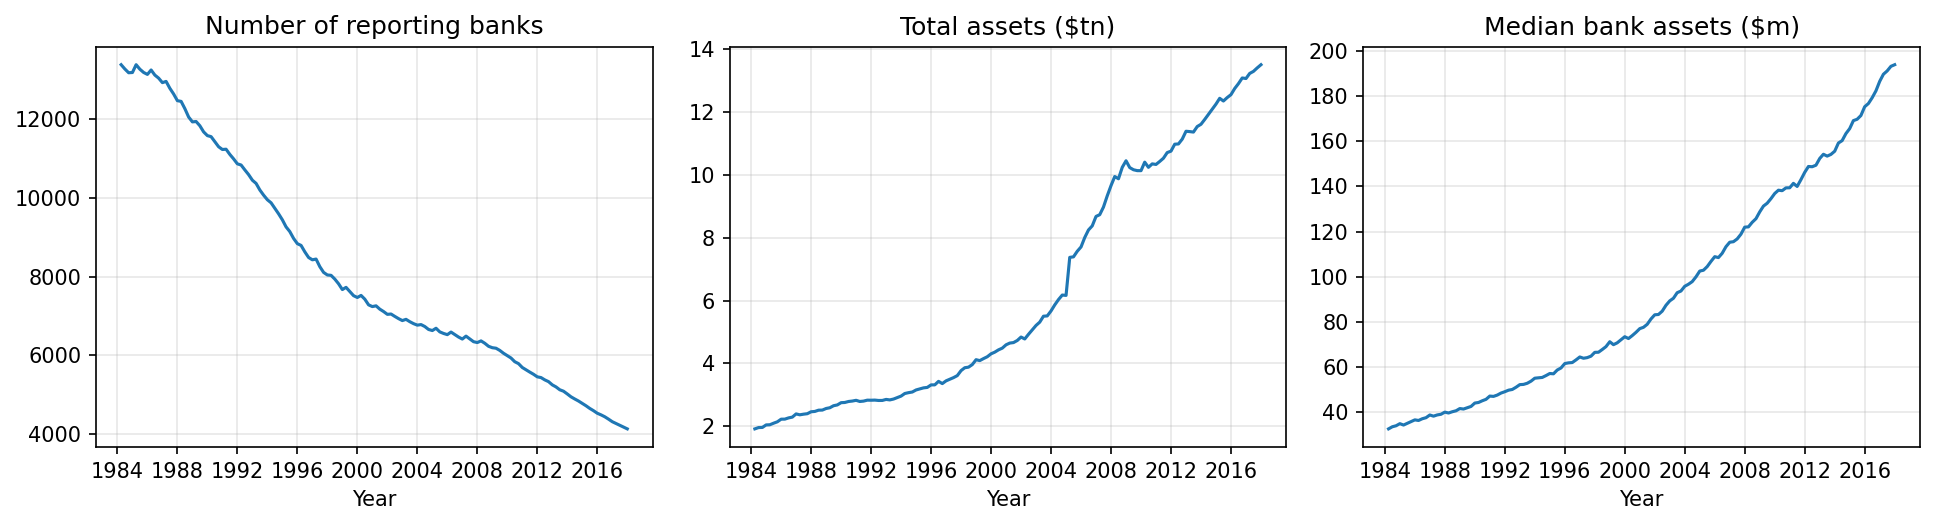
\includegraphics[width=0.72\textwidth]{output/figures/fig1_industry_over_time.png}
\caption{Banking industry over time: number of reporting banks (left), total
assets (center), median bank assets (right).}\label{fig:industry}
\end{figure}

\begin{figure}[H]\centering
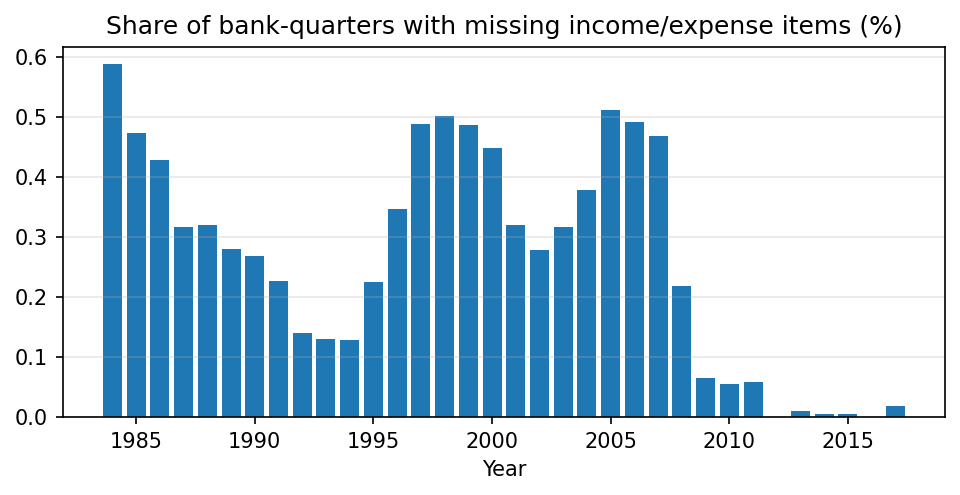
\includegraphics[width=0.62\textwidth]{output/figures/fig2_missing_values.png}
\caption{Share of bank-quarters with missing income/expense/net-income items by
year, computed on the raw panel before dropping rows.}\label{fig:miss}
\end{figure}

\begin{figure}[H]\centering
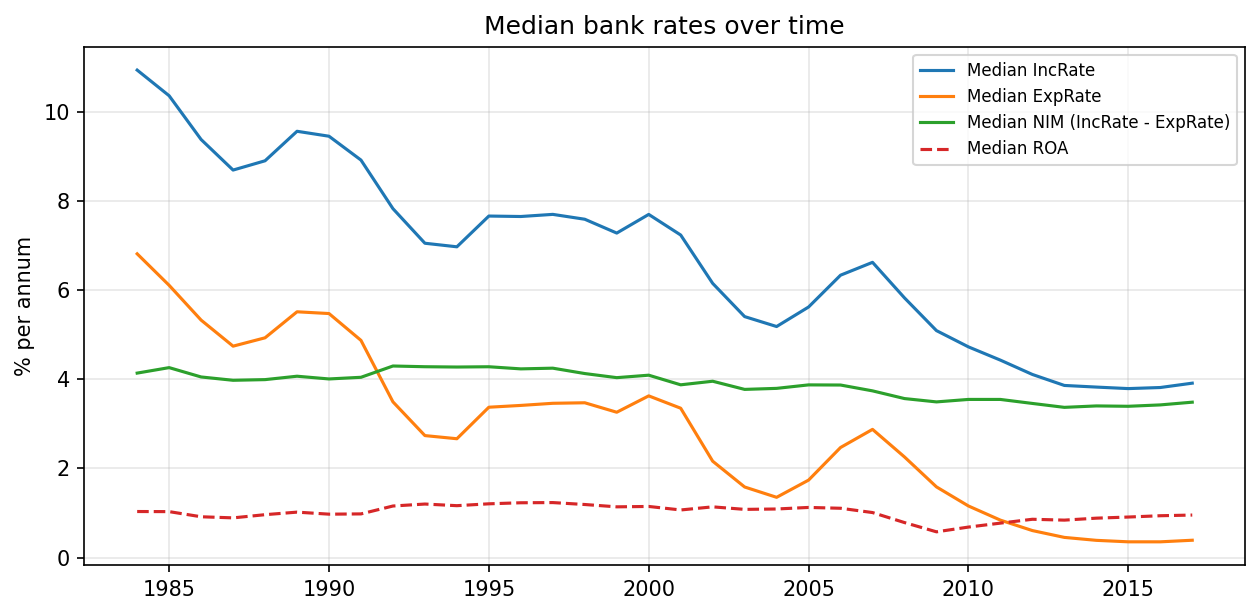
\includegraphics[width=0.8\textwidth]{output/figures/fig3_rate_trends.png}
\caption{Annual median IncRate, ExpRate, net interest margin (IncRate minus
ExpRate), and median ROA, 1984--2017. The margin is remarkably stable near
4 percentage points; ROA dips in 1987, 1991, and 2008--09.}\label{fig:trends}
\end{figure}

\subsection{Main patterns}
Three patterns stand out. First, the industry consolidated sharply: reporting
banks fell from about 13,500 in 1984 to about 4,500 by 2016, while total assets
grew more than sixfold (Figure~\ref{fig:industry}). Second, the
size distribution stayed extremely skewed (mean assets \$757m, median \$66m).
Third, the net interest margin hovered near 4 percentage points for the whole
sample, while median ROA moved with the cycle (Figure~\ref{fig:trends}).

Two data limitations matter for what follows. The panel is unbalanced and exit
is correlated with size, so time-series aggregates mix entry, exit, and
organic change. And the YTD reporting convention, if left untreated, would put
a mechanical seasonal component into every rate and every beta; the
reconstruction in the previous subsection is the main guard against that.

\section{Bank-Level Interest Income and Expense Betas}

For bank $i$ in quarter $t$ I construct annualized rates in percentage
points:

\begin{equation}
\begin{aligned}
\text{IncRate}_{i,t}&=400\times\frac{\text{interest income}_{i,t}}{\text{average assets}_{i,t}},\\
\text{ExpRate}_{i,t}&=400\times\frac{\text{interest expense}_{i,t}}{\text{average assets}_{i,t}}.
\end{aligned}
\end{equation}

using the reconstructed single-quarter flows. The federal funds rate
$f_t$ is the last monthly value of quarter $t$. First differences are

\begin{equation}
\Delta y_{i,t}=y_{i,t}-y_{i,t-1},\qquad \Delta f_t=f_t-f_{t-1},
\end{equation}

and, for each bank and each outcome $y\in\{\text{IncRate},\text{ExpRate},
\text{ROA}\}$, I estimate

\begin{equation}
\Delta y_{i,t}=a_i^y+\sum_{\tau=0}^{3}b_{i,\tau}^{y}\,\Delta f_{t-\tau}+u_{i,t}^y,
\end{equation}

with the four coefficients allowing the response to build over one year.
The bank's beta is the sum of the four estimated coefficients,

\begin{equation}
\widehat{\beta}_i^y=\sum_{\tau=0}^{3}\widehat{b}_{i,\tau}^{y}.
\end{equation}

I require at least 20 usable first-difference observations per bank
(about five years). This gives 13,624 eligible banks of 17,743 (77\%); most
excluded banks are short-lived or de novo. Median one-year betas are 0.358 for
income and 0.353 for expense. A one-percentage-point rise in the federal funds
rate is associated, within a year, with about a 0.36-point rise in the income
rate and a 0.35-point rise in the expense rate. The ROA beta distribution is
centered near zero (median -0.012, SD 0.70), so profitability is only loosely
tied to rate movements on average (Table~\ref{tab:t2}, Figure~\ref{fig:betadist}).

\begin{table}[H]\centering\small
\caption{Distribution of bank-level estimated betas (13,624 banks). Rates are
winsorized at 0.5/99.5 within quarter; the \_w suffix is dropped in the text
and tables. Betas are not trimmed further.}\label{tab:t2}
\begin{tabular}{lccc}\toprule
Statistic & Beta\_Inc & Beta\_Exp & Beta\_ROA\\
\midrule
N banks & 13624 & 13624 & 13624\\
Mean & 0.369 & 0.354 & -0.014\\
SD & 0.276 & 0.145 & 0.703\\
p10 & 0.183 & 0.230 & -0.360\\
p25 & 0.269 & 0.294 & -0.134\\
Median & 0.358 & 0.353 & -0.012\\
p75 & 0.464 & 0.418 & 0.114\\
p90 & 0.594 & 0.492 & 0.363\\
\bottomrule
\end{tabular}
\end{table}

\begin{figure}[H]\centering
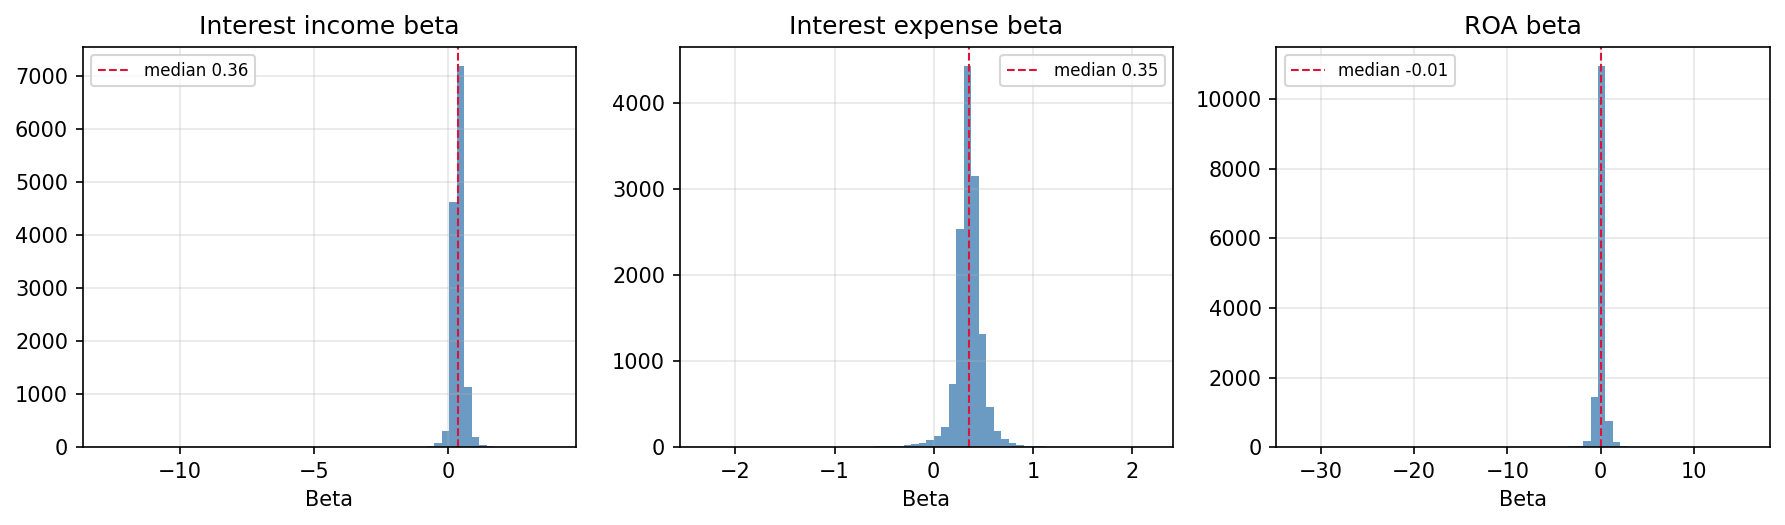
\includegraphics[width=0.85\textwidth]{output/figures/fig4_beta_distributions.png}
\caption{Histograms of bank-level income, expense, and ROA betas. The ROA
distribution is much wider than the two rate betas.}\label{fig:betadist}
\end{figure}

The cleaned bank-level dataset is submitted as
\texttt{data\_processed/bank\_betas.csv}: one row per bank (17,743 rows) with
idrssd, bank name, first/last quarter, mean assets, the three betas
(beta\_Inc, beta\_Exp, beta\_ROA), observation counts, R$^2$, and eligibility
flags. Banks below the 20-observation minimum keep a row with missing betas,
so the file contains every bank in the panel. Size in that file is each
bank's time-series average of total assets over its usable sample
(mean\_asset), the natural one-row-per-bank analogue of the quarterly asset
measure.

\section{Relationship between Income and Expense Sensitivities}

I regress income beta on expense beta by OLS:

\begin{equation}
\widehat{\beta}_i^{\text{Inc}}=\alpha+\gamma\,\widehat{\beta}_i^{\text{Exp}}+\varepsilon_i.
\end{equation}

I use HC1 heteroskedasticity-robust standard errors for the
cross-sectional regressions. The estimates are based on one observation per
bank; the table reports coefficients, HC1 t-statistics, sample sizes, and
adjusted R-squared values.

\begin{table}[H]\centering\small
\caption{Cross-sectional regressions of income beta on expense beta (Panel A)
and ROA beta on expense beta (Panel B), one observation per bank. HC1
t-statistics in parentheses. Size terciles are defined by each bank's
time-series average total assets (mean\_asset), not within-quarter assets.
For interaction rows, `Slope' is the expense-beta coefficient at average log
assets; the level term in log assets is not shown. Stars denote two-sided
significance at 10\%, 5\%, and 1\% (*, **, ***).}\label{tab:t3}
\begin{tabular}{llllll}\toprule
Specification & Intercept & Slope & N & Adj R2 & Interaction\\
\midrule
A: Inc on Exp (full) & 0.116$^{***}$ (3.76) & 0.715$^{***}$ (8.17) & 13624 & 0.14 & \\
B: ROA on Exp (full) & -0.257$^{**}$ (-2.11) & 0.688$^{**}$ (2.03) & 13624 & 0.02 & \\
A: Inc on Exp, Small & 0.174$^{***}$ (13.53) & 0.529$^{***}$ (14.16) & 4541 & 0.117 & \\
A: Inc on Exp, Medium & 0.087$^{**}$ (2.08) & 0.797$^{***}$ (6.92) & 4541 & 0.213 & \\
A: Inc on Exp, Large & 0.097 (1.25) & 0.777$^{***}$ (3.76) & 4542 & 0.114 & \\
B: ROA on Exp, Small & -0.092$^{***}$ (-2.59) & 0.165$^{*}$ (1.66) & 4541 & 0.001 & \\
B: ROA on Exp, Medium & -0.478 (-1.44) & 1.323 (1.43) & 4541 & 0.05 & \\
B: ROA on Exp, Large & -0.188 (-1.48) & 0.521 (1.53) & 4542 & 0.013 & \\
A: interaction with log assets & 0.115$^{***}$ (3.84) & 0.707$^{***}$ (9.45) & 13624 & 0.147 & 0.092 (0.76)\\
B: interaction with log assets & -0.258$^{**}$ (-2.06) & 0.687$^{**}$ (2.01) & 13624 & 0.02 & 0.027 (0.16)\\
\bottomrule
\end{tabular}
\end{table}

The estimated slope is positive and below one (Table~\ref{tab:t3},
Panel A): a 0.1 higher expense beta corresponds to about a 0.072 higher income
beta. This is consistent with asset and liability repricing moving together,
while income rates respond less than one-for-one on average. The positive
intercept indicates that banks with low expense sensitivity can still have
positive income sensitivity, as would be expected when some assets reprice
with short-term rates.

The relationship is positive in each size tercile, with a somewhat larger
slope among medium and large banks than among small banks. The interaction
between expense beta and demeaned log assets is not statistically significant;
the data do not show a clear linear size gradient (Figure~\ref{fig:incexp}).

\begin{figure}[H]\centering
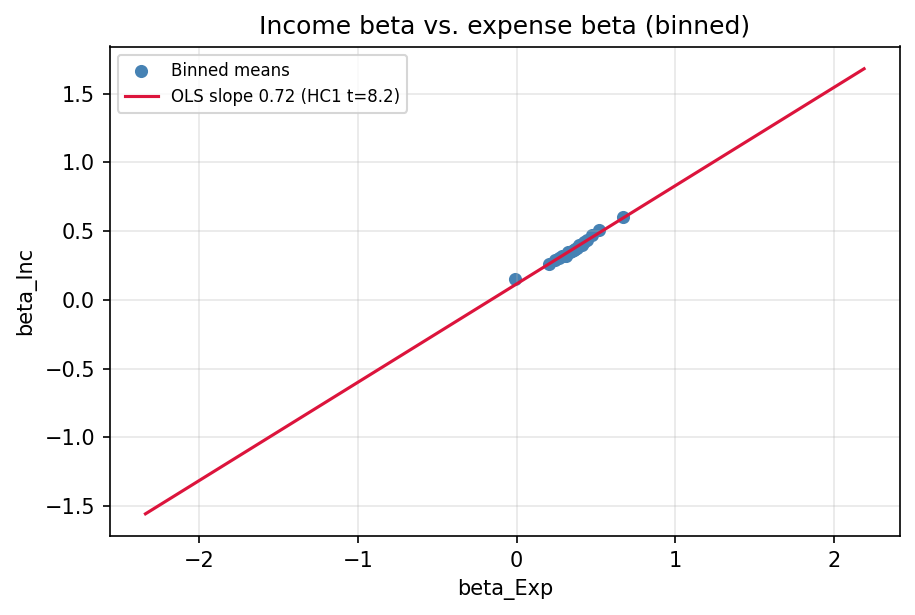
\includegraphics[width=0.62\textwidth]{output/figures/fig5_inc_vs_exp.png}
\caption{Binned scatter of income beta against expense beta (20
equal-frequency bins) with the OLS line. All eligible banks are included.}
\label{fig:incexp}
\end{figure}

\section{Interest Sensitivity of Profitability}

ROA is net income divided by average assets, annualized:

\begin{equation}
\text{ROA}_{i,t}=400\times\frac{\text{quarterly net income}_{i,t}}
{\text{quarterly average assets}_{i,t}},
\end{equation}

and the ROA beta comes from the same distributed-lag regression. Regressing
beta\_ROA on beta\_Exp gives a positive slope (HC1 t = 2.03), with adjusted
R$^2$ = 0.020 (Table~\ref{tab:t3}, Panel B). Expense beta explains only a
small share of cross-bank variation in ROA beta. The negative intercept is
hard to interpret mechanically because very few banks have exactly zero
expense sensitivity.

\begin{figure}[H]\centering
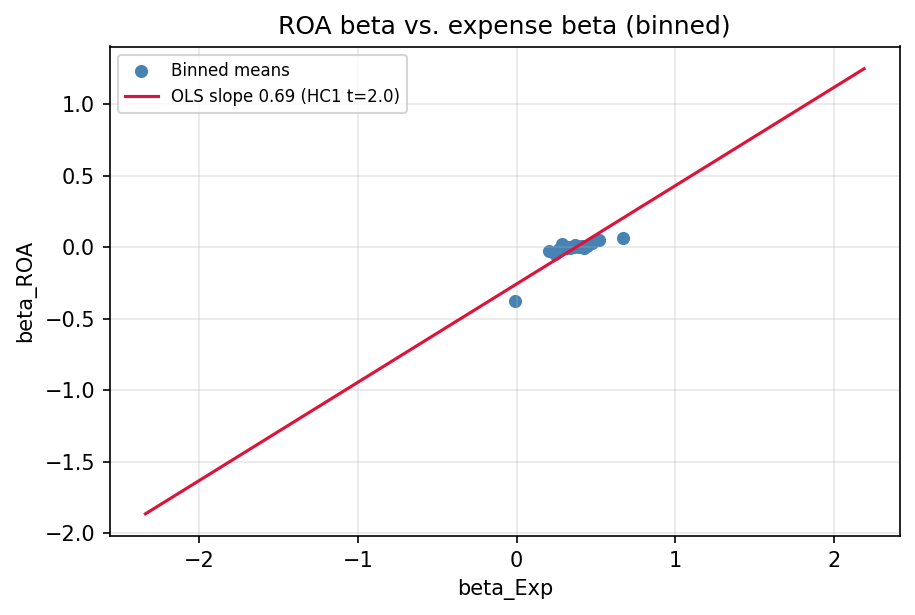
\includegraphics[width=0.62\textwidth]{output/figures/fig6_roa_vs_exp.png}
\caption{Binned scatter of ROA beta against expense beta with the OLS line.
The positive slope is driven mostly by the upper bins; the fit is weak
everywhere (R$^2$ = 0.02).}\label{fig:roaexp}
\end{figure}

Size heterogeneity: the estimated slopes are positive across size groups,
but none is statistically distinguishable from zero at conventional levels.
The interaction with demeaned log assets is also insignificant
(Figure~\ref{fig:roaexp}). The overall message of this section is that profitability
sensitivity is weakly related to expense sensitivity, with most cross-bank
variation left unexplained.

\section{Publicly Traded Banks}\label{sec:stocks}

\subsection{Linking banks to stocks}
I map the bank panel to CRSP with \texttt{Bank\_and\_CRSP\_Linking\_Table.csv},
which links RSSD identifiers (bank idrssd, holding-company rssd9001) to
PERMCO. Matching is on the bank's own idrssd first; banks with no idrssd match
are then tried through the holding company's bhc\_id. I chose this order after
checking that a naive concat of the two match types could put the same bank
under two different PERMCOs and double-count its assets and flows in the
company aggregates. Each link is restricted to its validity window
[dt\_start, dt\_end]. This yields 124,929 bank-quarter links covering 5,163
banks and 1,062 listed companies (PERMCO). No bank-quarter has multiple
PERMCOs among the valid links.

Where several banks map to one company, I aggregate to the company level:
average assets, total assets, and the three quarterly flows are summed
(stocks and flows both aggregate linearly), and the rates are recomputed from
the sums. These records include only banks matched to a listed company, so
company assets and flows may be understated when subsidiaries are unmatched;
ambiguous links are excluded. Intra-company transfers are not netted out, and
partly owned subsidiaries are counted at 100\% rather than by ownership share.
Call Report data do not let me separate these components, so the resulting
consolidated rates may be biased.

\subsection{Total-return index}
CRSP lists multiple share classes (PERMNO) for the same company-month. Before
building any series I collapsed them using prior-month market-cap weights, so
a company's monthly return is the value-weighted average of its share classes.
The CRSP file contains 453,756 PERMCO-month duplicates from multiple share classes. Monthly returns use
MthRet, which includes dividends, so the compounded series is a total-return
index (2000 = 100).

\begin{figure}[H]\centering
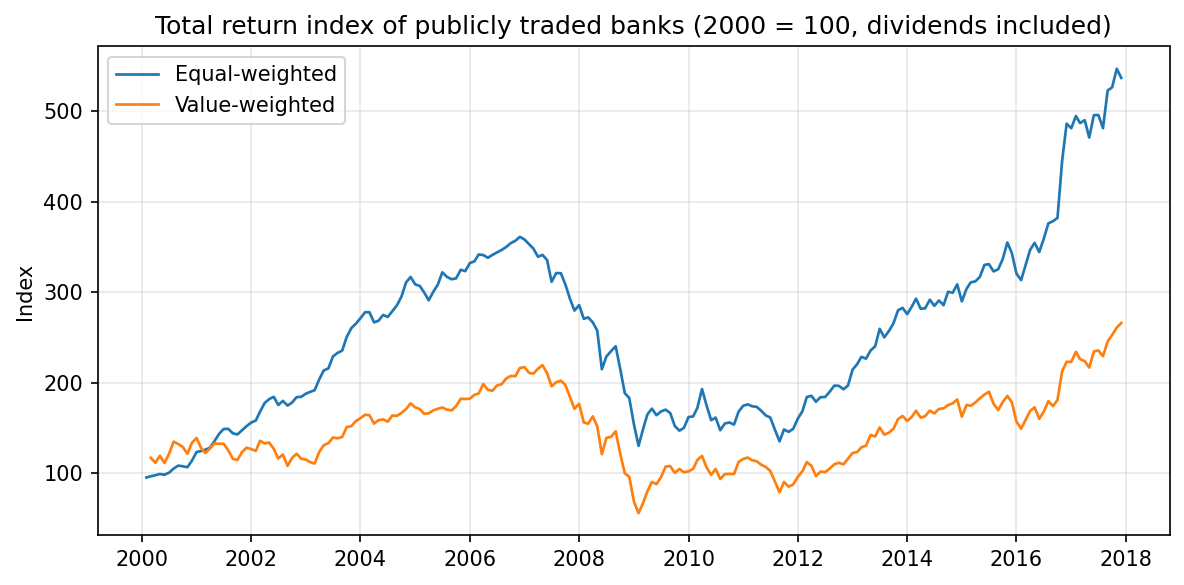
\includegraphics[width=0.72\textwidth]{output/figures/fig7_bank_stock_index.png}
\caption{Total return index of publicly traded banks (2000 = 100, dividends
included), equal-weighted and value-weighted, 2000--2017. The value-weighted
index lost about 60\% peak-to-trough in 2008--09; the equal-weighted index
fell far less, so most crisis losses were concentrated in the big
banks.}\label{fig:index}
\end{figure}

Figure~\ref{fig:index} shows that the value-weighted index fell much more
during 2008--09 and recovered more slowly than the equal-weighted index.
Returns among the largest listed bank companies drove much of the
value-weighted series' decline.

\subsection{Bank characteristics and stock returns}
To avoid look-ahead bias, each quarter's Call Report is treated as public two
months after quarter end (reports are filed with a lag); each monthly return
is matched to the most recent report whose public date is no later than that
month. The company-level expense beta is not used in return regressions
because a full-sample beta would embed post-return information; return tests
use only lagged accounting levels. After aggregation, company-level IncRate,
ExpRate, and ROA are recomputed from summed flows and assets, then winsorized
at the 0.5/99.5 percentiles within quarter. This applies the same percentile
cutoffs as the bank-level rates while defining outliers across linked
companies.

\begin{table}[H]\centering\small
\caption{Monthly stock returns of listed banks on lagged company
characteristics, 2000--2017. Coefficient (t-statistic clustered by listed
company). vwretd is the CRSP value-weighted market return; company rates are
winsorized within quarter. Stars denote two-sided significance at 10\%, 5\%,
and 1\% (*, **, ***).}\label{tab:t4}
\begin{tabular}{lccc}\toprule
Variable & (1) Market & (2) +Size+ROA & (3) +Rates\\
\midrule
Constant & 0.0053$^{***}$ (12.54) & 0.0123$^{***}$ (3.62) & 0.0023 (0.57)\\
Market return (vwretd) & 0.6137$^{***}$ (36.62) & 0.6169$^{***}$ (36.87) & 0.6148$^{***}$ (36.69)\\
Log total assets &  & -0.0006$^{***}$ (-2.80) & -0.0005$^{**}$ (-2.43)\\
ROA (\%) &  & 0.0024$^{***}$ (4.10) & 0.0020$^{***}$ (3.64)\\
Income rate (\%) &  &  & 0.0030$^{***}$ (5.33)\\
Expense rate (\%) &  &  & -0.0041$^{***}$ (-5.27)\\
N & 77720 & 77720 & 77720\\
R-squared & 0.0592 & 0.0606 & 0.0612\\
\bottomrule
\end{tabular}
\end{table}

The market-return coefficient is positive and precisely estimated. Conditional
on the market return, larger company-level assets are associated with slightly
lower subsequent monthly returns. In the rate specification, income rate
enters positively and expense rate negatively, consistent with a positive
association between net interest margins and subsequent returns
(Table~\ref{tab:t4}). All three specifications use the same 77,720
company-month observations.

\section{Is the Pass-Through of Policy Rates to Bank Funding Costs Symmetric?}

\subsection{Empirical approach}
Section 2 estimated a single expense beta, implicitly assuming that funding costs
respond symmetrically to rate increases and decreases. Deposit rates are often
described as sticky downward: banks reprice deposits quickly when the Fed
raises, but cut them slowly when the Fed lowers. If so, a cut in the policy
rate should pass through to funding costs less than a hike of the same size,
widening margins during easing cycles. I test this directly by splitting each
quarterly change in the federal funds rate into an increase and a decrease
part,

\begin{equation}
\Delta f^{+}_t=\max(\Delta f_t,0),\qquad
\Delta f^{-}_t=\min(\Delta f_t,0),
\end{equation}

and estimating, for each bank,

\begin{equation}
\Delta \text{ExpRate}_{i,t}=a_i+\sum_{\tau=0}^{3}b^{\text{up}}_{i,\tau}\,\Delta f^{+}_{t-\tau}
+\sum_{\tau=0}^{3}b^{\text{down}}_{i,\tau}\,\Delta f^{-}_{t-\tau}+u_{i,t},
\end{equation}

with the two cumulative betas

\begin{equation}
\beta^{\text{up}}_{i}=\sum_{\tau=0}^{3}\widehat{b}^{\text{up}}_{i,\tau},\qquad
\beta^{\text{down}}_{i}=\sum_{\tau=0}^{3}\widehat{b}^{\text{down}}_{i,\tau}.
\end{equation}

The identification compares how a bank's expense rate moves in quarters
following rate hikes versus quarters following rate cuts, over the same
distributed-lag window as in Section 2. I require at least 28 usable observations
(seven years), leaving at least 19 residual degrees of freedom after estimating
eight lag coefficients and an intercept. The table reports the eligible sample
sizes. Size terciles use each bank's time-series mean of total assets, as in
Section 3. Estimated betas are not trimmed. All results are descriptive, not causal.

\begin{table}[H]\centering\scriptsize
\caption{Asymmetry in interest-expense pass-through. Mean difference is
$\beta_{up}-\beta_{down}$; positive values mean greater pass-through during
hikes. Share reports the fraction of banks with a positive difference.}
\label{tab:t5}
\setlength{\tabcolsep}{2.5pt}
\begin{tabular}{lrrrrrrrr}\toprule
Sample & N & Mean up & Mean down & Mean diff. & Median diff. & Share with diff $>0$ & Paired t & p-value\\
\midrule
Full sample (1984-2017) & 12242 & 0.385 & 0.355 & +0.029 & +0.006 & 51.2\% & 7.61 & <0.001\\
Small & 4081 & 0.322 & 0.352 & -0.030 & -0.026 & 43.6\% & -5.23 & <0.001\\
Medium & 4080 & 0.386 & 0.351 & +0.035 & +0.004 & 50.8\% & 5.14 & <0.001\\
Large & 4081 & 0.445 & 0.364 & +0.082 & +0.036 & 59.3\% & 11.70 & <0.001\\
Pre-2007 (re-estimated) & 11403 & 0.352 & 0.402 & -0.050 & -0.060 & 35.6\% & -17.17 & <0.001\\
\bottomrule
\end{tabular}
\end{table}

\begin{figure}[H]\centering
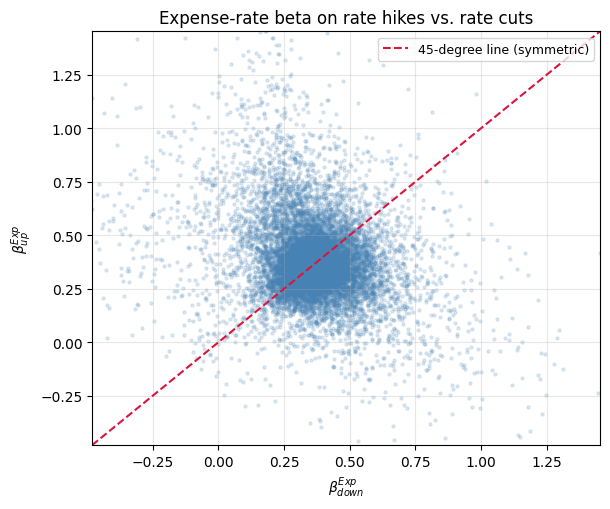
\includegraphics[width=0.62\textwidth]{output/figures/fig8_asym_scatter.png}
\caption{Bank-level cumulative expense-rate betas for rate hikes and cuts. The dashed line shows equal pass-through; axes show the central 99\% of estimates. All eligible banks enter the summary table.}
\label{fig:asymscatter}
\end{figure}

\begin{figure}[H]\centering
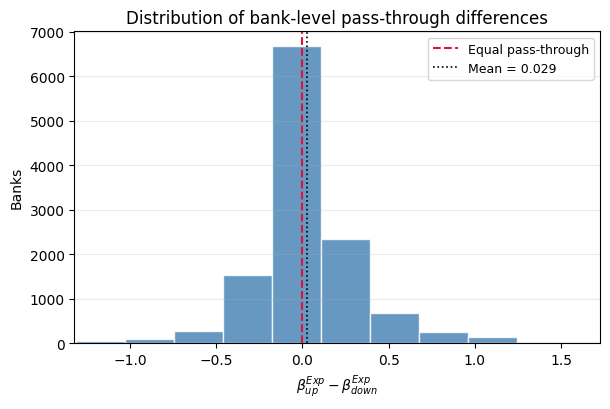
\includegraphics[width=0.68\textwidth]{output/figures/fig9_asym_diff.png}
\caption{Distribution of full-sample bank-level differences,
$\beta_{up}-\beta_{down}$. Axes show the central 99\% of estimates; all
banks are included in the table. The dashed line marks zero and the dotted
line marks the sample mean.}
\label{fig:asymdiff}
\end{figure}

\subsection{Results}
Table~\ref{tab:t5} reports the mean hike-minus-cut difference with its sign
shown explicitly. In the full sample it is +0.029; the pre-2007 re-estimate is -0.050. The sign reversal means the full-sample result does not show a stable asymmetry across periods. Figure~\ref{fig:asymscatter} compares the two betas directly, while Figure~\ref{fig:asymdiff} shows the distribution of their differences.

By size, mean differences are -0.030, +0.035, and +0.082 for small, medium, and large banks, respectively. These descriptive tercile comparisons do not establish a causal size pattern.

The sign has a direct interpretation: if $\beta_{up}>\beta_{down}$, expense rates pass through more during hikes, consistent with slower adjustment during cuts; if the two betas are equal, pass-through is symmetric; if $\beta_{down}>\beta_{up}$, pass-through is greater during cuts. Moreover, aggregate interest expense includes more than deposit costs, so this measure does not identify deposit pricing. Nor does the comparison by itself establish how net interest margins move, because asset yields also reprice. Hikes and cuts differ in number and size, bank-level betas are estimated with noise, and the results apply to banks meeting the 28-observation minimum. These estimates are descriptive, not causal.

\section{Conclusion}
Income and expense rates respond positively to federal funds rate changes,
and their bank-level betas move together. Profitability betas are only weakly
related to expense betas. In the stock-return regressions, the market return
is strongly associated with bank stock returns; accounting-rate associations
are modest. The hike-minus-cut difference is positive in the full sample
but negative in the pre-2007 re-estimation, so the evidence does not support a
stable asymmetry across periods. All findings are descriptive, not causal.

\clearpage
\appendix
\section{Reproducible Code}
All seven scripts are released with this report. They read the four raw files
(Call Report, federal-funds series, bank--CRSP link table, CRSP monthly stock
file) from \texttt{data/}, write processed data to \texttt{data\_processed/},
and write tables and figures to \texttt{output/}; run them in the order shown.
The code is reproduced here verbatim, with line numbers.

\lstinputlisting[language=Python,caption={\texttt{01\_data\_prep.py} \textemdash\ Read the raw Call Report, undo YTD cumulation, annualize and winsorize the rates, and build the bank-quarter panel, descriptive table, and data-audit figures.},captionpos=t]{code/01_data_prep.py}
\lstinputlisting[language=Python,caption={\texttt{02\_estimate\_betas.py} \textemdash\ Estimate bank-level interest-income, interest-expense, and ROA betas by a distributed-lag regression on federal-funds changes.},captionpos=t]{code/02_estimate_betas.py}
\lstinputlisting[language=Python,caption={\texttt{02b\_asym\_betas.py} \textemdash\ Split federal-funds changes into positive and negative parts and estimate asymmetric expense betas for the full and pre-2007 samples.},captionpos=t]{code/02b_asym_betas.py}
\lstinputlisting[language=Python,caption={\texttt{03\_cross\_section.py} \textemdash\ Cross-sectional regressions of income and ROA betas on expense beta, with mean-assets terciles and a demeaned log-asset interaction.},captionpos=t]{code/03_cross_section.py}
\lstinputlisting[language=Python,caption={\texttt{04\_stock\_link.py} \textemdash\ Link banks to CRSP PERMCOs, aggregate share classes by prior-month market cap, build the total-return index, and run stock-return regressions.},captionpos=t]{code/04_stock_link.py}
\lstinputlisting[language=Python,caption={\texttt{05\_q2\_extension.py} \textemdash\ Summarize and plot the hike-versus-cut asymmetry, with paired tests and size terciles for the full and pre-2007 samples.},captionpos=t]{code/05_q2_extension.py}
\lstinputlisting[language=Python,caption={\texttt{06\_make\_report.py} \textemdash\ Compile this report and append the code listings (this PDF).},captionpos=t]{code/06_make_report.py}
\end{document}
